\section{HTTP Method Request}
\subsection{Pengertian HTTP Method Request}
\subsection {Mekanisme HTTP Method Request}
\subsection {Contoh URL HTTP Get Method}
\subsection {Mendapatkan Parameter GET Python Flask}
    \begin{enumerate}
        \item Pengenalan Python

        Python adalah salah satu bahasa pemograman tingkat tinggi yang bersifat interpreter, interactive, objectoriented, dan dapat beroperasi hampir di semua platform: Mac, Linux, dan Windows. Python termasuk bahasa pemograman yang mudah dipelajari karena sintaks yang jelas, dapat dikombinasikan dengan penggunaan modulmodul siap pakai, dan struktur data tingkat tinggi yang efisien \cite{kadir2005dasar}. Python mendukung multi paradigma pemrograman, utamanya; namu tidak dibatasi; pada pemrograman berorientasi objek, pemrograman imperatif, dan pemrograman fungsional. Salah satu fitur yang tersedia pada python adalah sebagai bahasa pemrograman dinamis yang dilengkapi dengan manajemen memori otomatis.

        Seperti halnya pada bahasa pemrogrman dinamis lainnya, python umumnya digunakan sebagai bahasa skrip meski pada praktiknya penggunaan bahasa ini lebih luas mencakup konteks pemanfaatan yang umumnya tidak dilakukan dengan menggunakan bahasa skrip. Python dapat digunakan untuk berbagai keperluan pengembangan perangkat lunak dan dapat berjalan di berbagai platform sistem operasi.

        \item Pengenalan Flask
        
         Flask adalah \textit{Web Application Framework} yang ditulis dalam bahasa pemrograman Python. Flask digunakan untuk mempersingkat dan mempermudah pengembangan \textit{Web Application}\cite{lokhande2015efficient}. Flask disebut micro framework karena tidak membutuhkan alat-alat tertentu atau pustaka. Flask tidak memiliki database abstraction layer, validasi form, atau komponen lain dimana sudah ada database pihak ketiga yang menyediakan fungsi umum.
         
        \item Penjelasan Parameter GET Python Flask
        
        Parameter GET pada Python Flask ini dilampurkan dan diujikan dalam bentuk file penuh dengan beberapa fungsi. File tersebut bernama Main.py. Untuk penerapan lebih dan contoh GETnya sudah ditampilkan dan dijelaskan sebelumnya pada point contoh URL GET. Namun, penggabungannya bersama Flask Python ada pada file ini. Perhatikan penjelasan dan tutorialnya agar dapat dimengerti. Namun sebelum melanjutkan tutorialnya, pertama-tama anda harus memastikan beberapa hal yaitu sebagai berikut :
        
    \end{enumerate}

\section{Macam-Macam Penanganan Error Proyek}

\subsection{Penanganan Error pada Python dan Flask}
\begin{enumerate}
  \item Contoh Kasus 1 : Penerapan fungsi sederhana yang dieksekusi dicommand prompt. Contoh pemanggilan fungsi apabila dieksekusi di CMD, seperti gambar \ref{fig:contohsederhana}

  \begin{figure}[!ht]
        \centerline{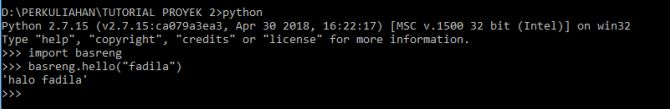
\includegraphics[width=0.70\textwidth]{figures/10/contohsederhana.jpg}}
	    \caption{Fungsi Sederhana}
	    \label{fig:contohsederhana}
  \end{figure}


ini adalah contoh untuk pengeksekusian file python yang berupa gunsi yang telah dibuat. Berikut langkah-langkahnya :
    \begin{itemize}
        \item Petama-tama masukkan kedalam directory tempat anda menyimpan file yang telah anda buat.
        \item kemudian pada directory tersebut ketik python
        \item Setelah masuk kedalam python silahkan masukkan file python basreng
    \end{itemize}

  \item Contoh kasus 2 : Kode pembawa sinyal gelombang otak (NeuroSky Mindwave EEG). Kodenya seperti contoh \ref{lst:coba}, silahkan tutorialnya diikuti terlebih dahulu.
\lstinputlisting[caption=Contoh kode untuk membaca sinyal gelombang otak,label={lst:coba}]{src/10/coba.py}
\end{enumerate}

